\documentclass{scrartcl}
\usepackage{syntonly,graphicx,amssymb,amsmath,epsfig,lscape,fancyhdr,caption,subcaption}
\pagestyle{plain}
\usepackage[margin=1in]{geometry}
\begin{document}
\title{2G03: Numbers and Functions}
\author{AJM}
\maketitle
\begin{abstract}
This document details the rudimentary lessons learned in \textsc{C}.
It describes the following algorithms: \textsc{pi.c}, \textsc{sine.c}, \textsc{dist.c}, \textsc{interp.c}.
\end{abstract}
\section{Estimating $\pi$}
Euler proved two ways to compute $\pi$.
The first is a straight summation:
\begin{equation}
	\frac{\pi^{2}}{6}=\sum_{n=1}^{\infty}{\frac{1}{n^{2}}},
\end{equation}
but it converges very slowly.
He then showed that the following recursion relation also works:
\begin{align}
	\frac{\pi}{2}&=\sum_{n=1}^{\infty}{t_{n}} \\
	t_{n}&=t_{n-1}\frac{n-1}{2n-1}, t_{1}=1\notag
\end{align}
and it converges much more rapidly.
The recursion relation is truncated in \textsc{pi.c} when $t_{n}$ satisfies:
\begin{equation}
	t_{n}\leq\epsilon,
\end{equation}
where $\epsilon$ is user supplied and sets the error in the estimate: if we set $\epsilon$ as $10^{-2}$ and $10^{-4}$ respectively, we get $\Delta$ values of $9.4359\times10^{-3}$ and $1.1325\times10^{-4}$ with minimum terms $t_{7}=5.3280\times10^{-3}$ and $t_{13}=6.0588\times10^{-5}$.
Note that \textsc{pi.c} is written in single precision so $\Delta$ can only be accurately estimated for $\epsilon\gtrsim2\times10^{-7}$, with $t_{21}=1.8553\times10^{-7}$; the smallest $\epsilon$ one may set is $10^{-45}$ ($t_{146}=1.4013\times10^{-45}$).
The program has also been modified to not accept any number less than 0 (in single precision this is equivalent to setting $\epsilon<10^{-45}$).
\section{Taylor Series Approximation for sin(x)}
There are a number of series that return $\sin{x}$.
One simple method is to use a Taylor series expansion about the value $x=a$:
\begin{equation}
	f(x)=\sum_{i=0}^{\infty}{\frac{\rm{d}^{i}f(x)}{\rm{d}x^{i}}\frac{(x-a)^{i}}{i!}}
\end{equation}
truncated at some term (again, the error in the estimate is set by the truncation term).
In this program, the series is truncated in at the third term:
\begin{equation}
	\sin{x}\approx x-\frac{1}{6}x^{3}+\frac{1}{120}x^{5}+O(x^{7})
\end{equation}
where we have expanded about $x=0$.
The following table represents the estimates for four values of $x$ using the truncated Taylor expansion and that given by the sine function used in the standard \textsc{C} library $<math.h>$.
\begin{center}
	\begin{tabular}{|c|c|c|c|}\hline
		$x$ & $<math.h>$ & Taylor & $\Delta$ \\\hline
		0.5 & 0.479426 & 0.479427 & 0.000002 \\\hline
		1.0 & 0.841471 & 0.841667 & 0.000196 \\\hline
		2.0 & 0.909297 & 0.933333 & 0.024036 \\\hline
		4.0 & -0.756802 & 1.866667 & 2.623469 \\\hline
	\end{tabular}
\end{center}
The Taylor series approximation is only good around the value $a$; in this case, it performs horribly for values greater than 2.0.
Values greater than $\pi$ also presents problems since the Taylor series does not map onto the Cartesion unit circle.
In order to improve the estimate, the code has been modified to determine which quadrant $x$ lies in\footnote{It also ensures that values greater than 2$\pi$ are shifted to ensure periodicity.}, sets both $a$ and the sign appropriately, and then evaluates the series.
The resulting values are shown below.
\begin{center}
	\begin{tabular}{|c|c|c|c|}\hline
		$x$ & $<math.h>$ & Taylor & $\Delta$ \\\hline
		0.5 & 0.479426 & 0.479427 & 0.000002 \\\hline
		1.0 & 0.841471 & 0.841667 & 0.000196 \\\hline
		2.0 & 0.909297 & 0.909789 & 0.000491 \\\hline
		4.0 & -0.756802 & -0.756872 & 0.000069 \\\hline
	\end{tabular}
\end{center}
\section{Vectors using Structures}
The \textsc{dist} program computes the distance between two vectors in $\Re^{3}$ space.
The command line prompts for each vector component to be entered, separated by whitespace.
Once both vectors \textbf{D}$_{1}$ and \textbf{D}$_{2}$ are entered, the program returns $||$\textbf{D}$_{1}||$, $||$\textbf{D}$_{2}||$, and $||$\textbf{D}$_{2}-$\textbf{D}$_{1}||$.
The novelty is that rather than passing variables, it uses a structure system.
\section{Linear Interpolation}
The simplest interpolation scheme between two points $[x_{i},y_{i}]$ and $[x_{i+1},y_{i+1}]$ is to use a linear fit to the points at $x$:
\begin{equation}
	y\approx\frac{y_{i+1}-y_{i}}{x_{i+1}-x_{i}}x+x_{i}
\end{equation}
The quality of the interpolation depends on the how well a linear function approximates the function $y(x)$ between the sets of points.
The program uses \textsc{lookup.c} to search for the points that bracket the user supplied value for $x$ in order to calculate $y$.
Since the points are sorted, the lookup function is a simple for loop combined with an if statement.
It returns the location of the lower bracket, $i$, and passes it into \textsc{interp.c}.
Using $f(x)=\frac{3}{4}x^{2}+5$ as a test function yields the following results.
\begin{center}
   \begin{tabular}{|c|c|c|}\hline
		$x$ & $f(x)$ & $y$ \\\hline
		 0.52 &  5.2028 &   0.3900 \\\hline
		 3.75 & 15.5469 &  22.6875 \\\hline
		 4.31 & 18.9321 &  33.0925 \\\hline
		 9.99 & 79.8501 & 151.3575 \\\hline
		10.04 & 80.6012 & 168.1300 \\\hline
	\end{tabular}
\end{center}
\section{Numerical Calculus using Finite Differences}
The mathematical definition of a derivative is:
\begin{equation}
	\frac{\textrm{d}f}{\textrm{d}x}=\lim_{h\rightarrow 0}{\frac{f(x+h)-f(x)}{h}},
\end{equation}
while the integral is the limit of the Riemann sum:
\begin{equation}
	\int_{0}^{L}{f(x)\,\textrm{d} x}=\lim_{h\rightarrow 0}{\sum_{n=1}^{N}{f(x_{n})h}}.
\end{equation}
The method of finite differences uses these definitions to derive approximations --- that is, $h$ does not go to zero but is left at some finite value --- whose error can be derived from the appropriate Taylor approximation.
\subsection{Differentiation}
The first order approximation to calculate the numerical derivative of the function $f(x)$ is given by:
\begin{equation}
	\frac{\textrm{d}f}{\textrm{d}x}\approx\frac{f(x+\Delta x)-f(x)}{\Delta x}=\frac{\textrm{d}f}{\textrm{d}x}+\Delta x\frac{1}{2}\frac{\textrm{d}^{2}f}{\textrm{d}x^{2}}+O(\Delta x^{2})
\end{equation}
The leading error term is of order $\Delta x$ and scales as the second order derivative of the function.
As test, we use the following function:
\begin{align*}
	f(x)&=1-x+4x^{2}-x^{3} \\
	f'(x)&=-1+8x-3x^{2} \\
	f''(x)&=8-6x
\end{align*}
The root-mean-square of the difference in the integral at each point will be used to guage the error in the integral:
\begin{equation}
	\sigma_{rms}=\sqrt{\frac{1}{n}\sum_{i=1}^{n}{(\frac{f(x+\Delta x)-f(x)}{\Delta x}-\frac{\textrm{d}f}{\textrm{d}x})^{2}}}
\end{equation}
From the above definition of the numerical derivative, $\sigma_{rms}$ can be rewritten as:
\begin{align*}
\sigma_{rms}&=\sqrt{\frac{1}{n}\sum_{i=1}^{n}{(\Delta x\frac{1}{2}\frac{\textrm{d}^{2}f}{\textrm{d}x^{2}}+O(\Delta x^{2}))^{2}}}\\
	&\approx\sqrt{\frac{\Delta x^{2}}{4n}\sum_{i=1}^{n}{(\frac{\textrm{d}^{2}f}{\textrm{d}x^{2}})^{2}}}\\
	&\propto \frac{1}{n}
\end{align*}
This table below shows the result of differentiating $f(x)$ over the interval [0,1].
\begin{center}
	\begin{tabular}{c|ccccccccccc}
		$n$ & 10 & 20 & 30 & 40 & 50 & 60 & 70 & 80 & 90 & 100 \\\hline
		$\sigma_{rms}$ & 0.26917 & 0.13345 & 0.08871 & 0.06644 & 0.05310 & 0.04423 & 0.03789 & 0.03314 & 0.02946 & 0.02650
	\end{tabular}
\end{center}
As expected, a least squares fit shows that $\sigma_{rms}$ indeed goes as $n^{-1}$.
In Figure \ref{fig:diff} the error and $rms$ scaling are shown.
\begin{figure*}
	\centering
	\begin{subfigure}[b]{0.45\textwidth}
		\includegraphics[width=\textwidth]{deriv.ps}
		\caption{Differntial}
	\end{subfigure}
	\begin{subfigure}[b]{0.45\textwidth}
		\includegraphics[width=\textwidth]{derr.ps}
		\caption{Error}
	\end{subfigure}
	\label{fig:diff}
	\caption{Numerical differentiation.  Red symbols mark the $n=20$, blue for $n=40$, and green for $n=80$.}
\end{figure*}
\subsection{Integration}
We can write the approximate integral of $f(x)$ as:
\begin{equation}
	\int_{0}^{L}{f(x)\,\textrm{d} x}\approx\sum_{n=1}^{N}{f(x_{n})\Delta x}=\int_{0}^{L}{f(x)\,\textrm{d} x}+\Delta x^{2}\frac{L}{8}\frac{\textrm{d}^{2}f}{\textrm{d}x^{2}}+O(\Delta x^{3})
\end{equation}
where each point $x_{n}$ is given by $\Delta x(n-\frac{1}{2})$ --- the midpoint rule.
We can also write the $rms$ error as:
\begin{equation}
	\sigma_{rms}=\sqrt{\frac{1}{N}\sum_{i=1}^{N}{(\sum_{n=1}^{i}{f(x_{n})\Delta x}-\int_{0}^{x_{i}}{f(x)\,\textrm{d} x}})},
\end{equation}
which, like for the differential, can be rewritten as:
\begin{equation}
\sigma_{rms}\simeq\sqrt{\frac{1}{N}\sum_{i=1}^{N}{\Delta x^{2}\frac{L}{8}\frac{\textrm{d}^{2}f}{\textrm{d}x^{2}}}},
\end{equation}
where the higher order terms have been dropped.
This form also leads to the realization that to first order, $\sigma_{rms}$ should go as $n^{-1.5}$.
The figures below show the resulting integrand and the error in the integrand as a function of $n$.
\begin{figure*}
	\centering
	\begin{subfigure}[b]{0.45\textwidth}
		\includegraphics[width=\textwidth]{integ.ps}
		\caption{Integral}
	\end{subfigure}
	\begin{subfigure}[b]{0.45\textwidth}
		\includegraphics[width=\textwidth]{ierr.ps}
		\caption{Error}
	\end{subfigure}
	\label{fig:integ}
	\caption{Numerical integration.  The colours and symbols are the same as above.}
\end{figure*}
\begin{center}
	\begin{tabular}{c|ccccccccccc}
		$n$ & 10 & 20 & 30 & 40 & 50 & 60 & 70 & 80 & 90 & 100 \\\hline
		$\sigma_{rms}$ & 0.00147 & 0.00036 & 0.00016 & 0.00009 & 0.00006 & 0.00004 & 0.00003 & 0.00002 & 0.00002 & 0.00001
	\end{tabular}
\end{center}
\end{document}
